%************************************************
\chapter{Reference Implementation}\label{ch:implementation}
%************************************************

\autoref{ch:flexibleeventsubscription} has presented a concept that involves the model layer, the process engine and the event engine.
It enables flexible event subscription to overcome the issues revealed in ...
By explicitly chosing the time of event subscription and bridging the gap between event reception and consumption by the process instance it is possible to ...
\todo[inline]{write from keypoints}

the model extension is formalized in \autoref{ch:bpmnx}, hence BPMN models extended by all information necessary for flexible event subscription can be created.

to evaluate our results and provide a reference implementation, we enhance the business process engine Camunda and the event processing platform UNICORN following the procedures described in \autoref{ch:extendedprocessengine} and \autoref{ch:bufferedcep} respectively.
Camunda is extended by providing a Process Engine Plugin, Unicorn by adapting the source code.
The resulting illustration of an event-driven architecture is evaluated by implementing the examples shown in \autoref{ch:motivatingexamples}.

\begin{figure}[]
	\myfloatalign
	{\hspace*{-2.3cm}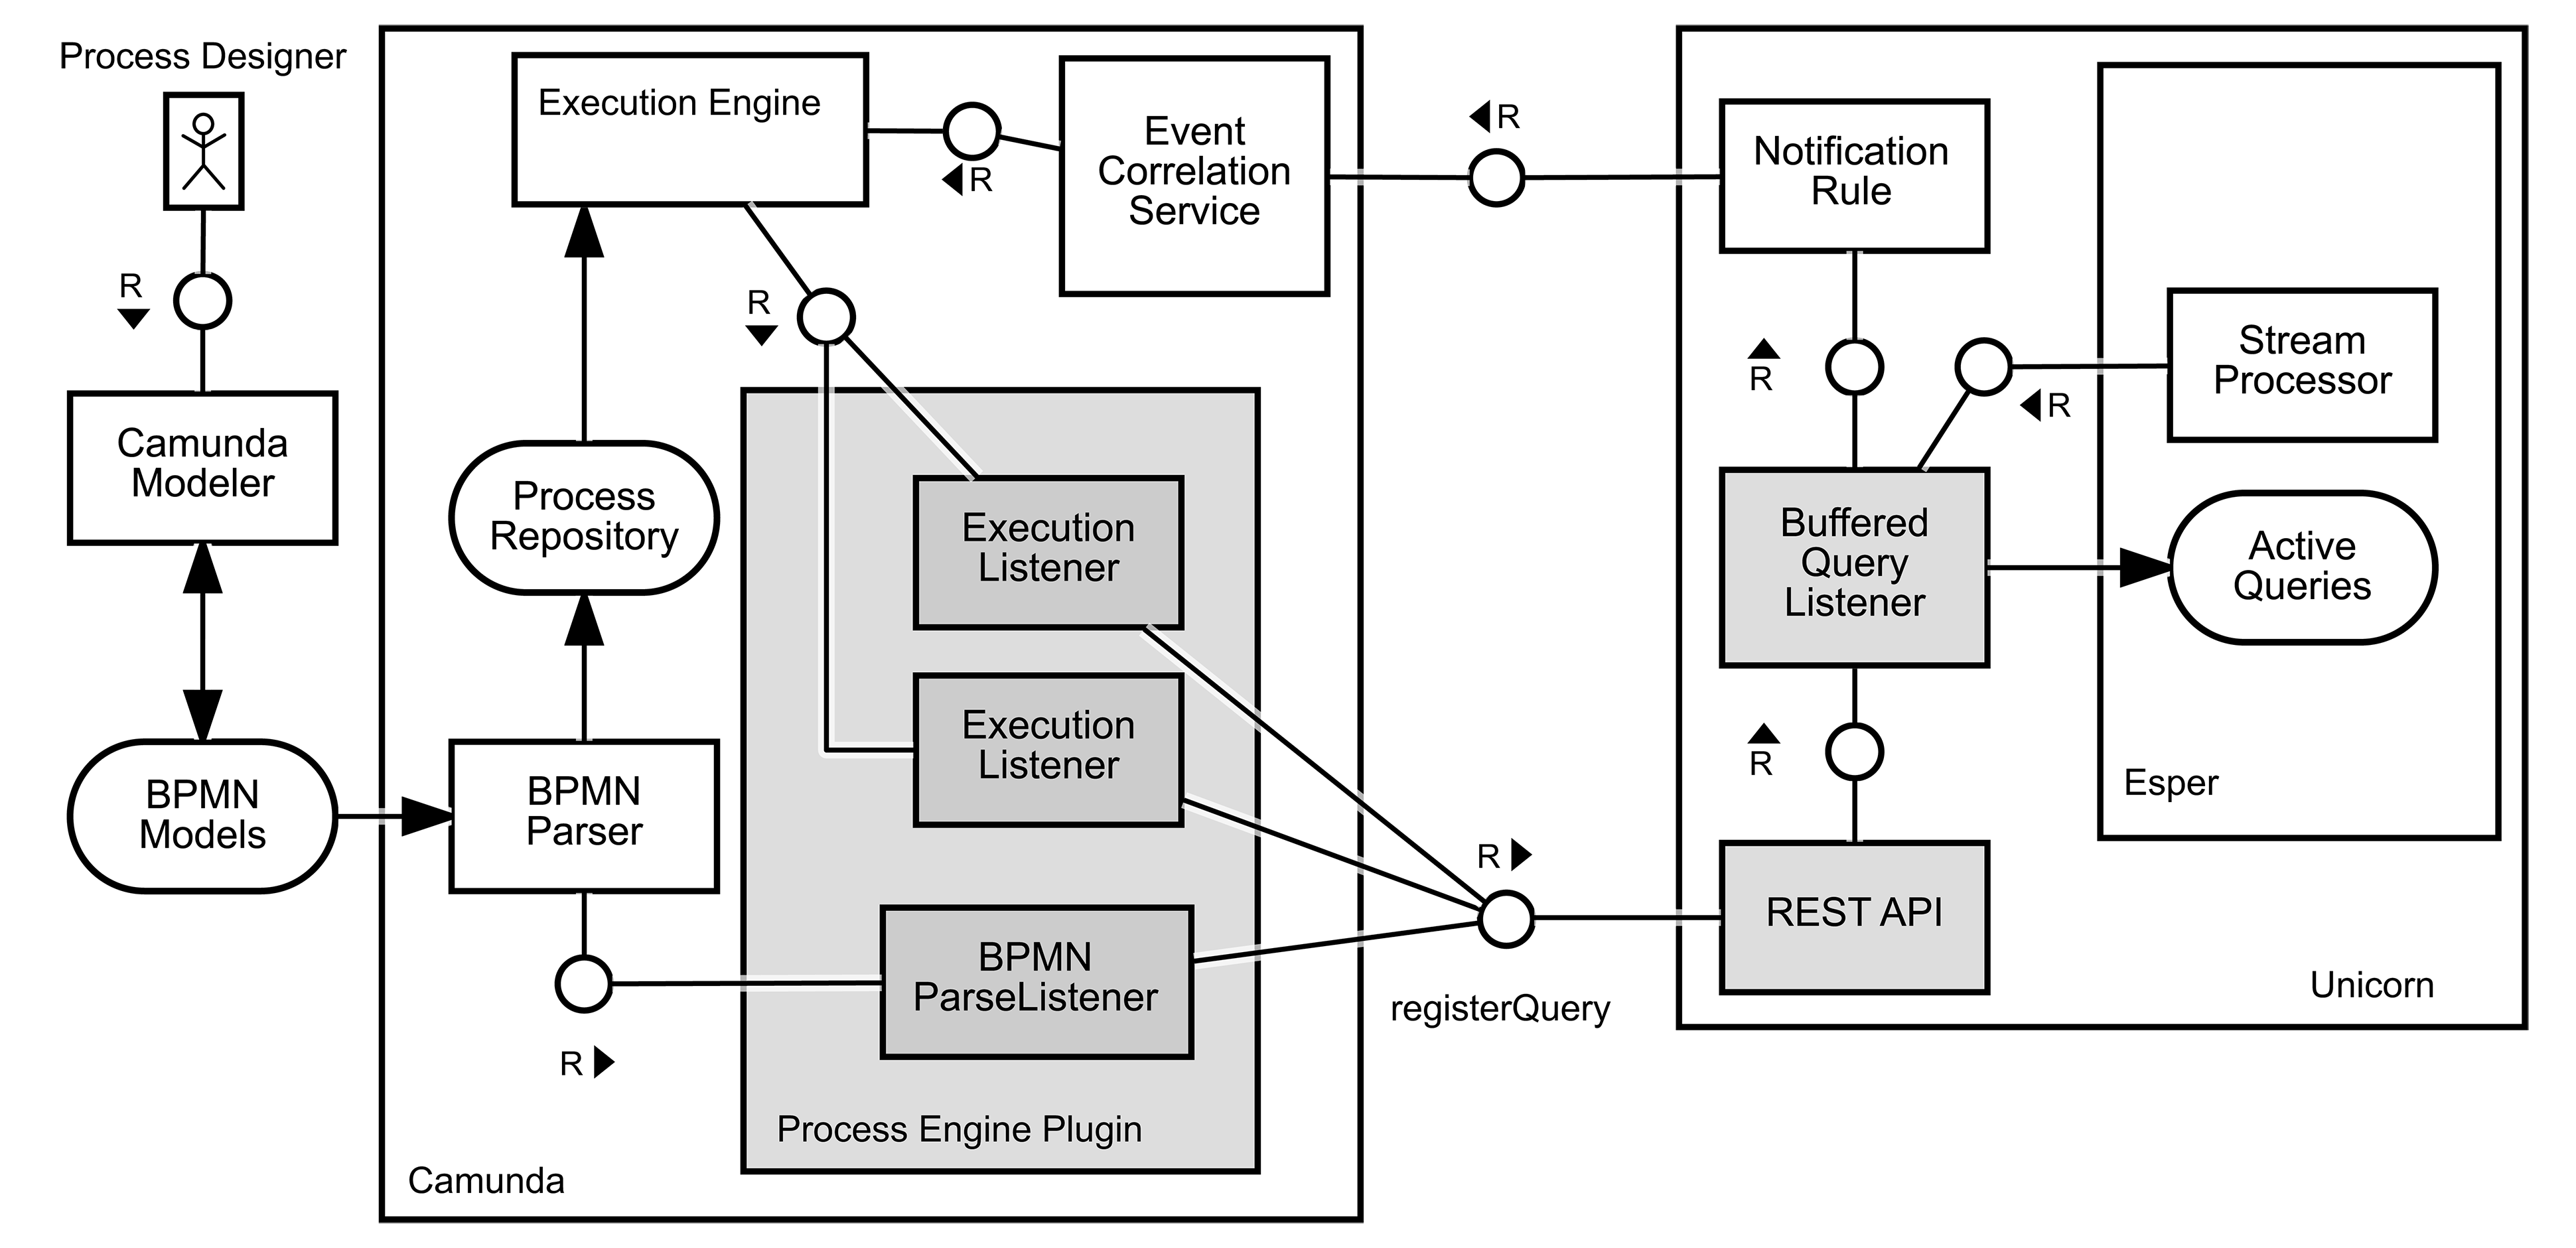
\includegraphics[width=1.3\linewidth]{chapters/implementation/flexible-evt-subscr-camunda-unicorn.png}}
	\caption{Architecture for flexible event subscription in Camunda and Unicorn}
	\label{fig:architecture-camunda-unicorn}
\end{figure}

\section{Extending the Event Processing Platform Unicorn}\label{ch:implunicorn}
\textit{UNICORN} is an event engine developed for academic purposes at the Business Process Technology chair of Hasso-Plattner-Institute, Potsdam.
\cite{herzberg2013event}
It focuses on event processing for \acs{BPM}, ...
Based on Esper, that means, what is esper
what unicorn adds to esper: graphical and rest user-interface to ..., event persistence store, bp execution and correlation, recently also an event generator/replayer
==> it translated user interactions into the according Esper method calls

- currently unicorn uses version 5.3.0 of esper, therefor all future considerations are made based on the documentation of that version
\todo[inline]{write from keypoints}

It has been decided to extend the event engine in this scenario, for several reasons.
Firstly, the performance and operation of the process engine shall not be jeopardized. Event Processing features potentially require a lot of performance to handle a large number of requests in a short amount of time.
By implementing the event Buffering module loosely coupled to the Process Engine, we ensure that its performance is not influenced.
Implementing a separate middleware was avoided in the course of this work, to keep the architecture easy and concise to describe.
Unicorn is an academic prototype in constant development and therefor predestined to be directly extended for this kind of use-case.
Moreover, the chosen architecture promises performance advantages thanks to running the event buffering in the same \acs{JVM} as Esper.


\subsection{Event Buffering}
To allow the delayed delivery of events, buffering functionality is added to Unicorn.
Whereas, originally, events that match a certain query in esper are directly forwarded to the notification-recipients, they will instead be held in a buffer until requested by recipient. 
If a recipient is already subscribed, than the behavior will be equivalent to the original scenario, because the event will be delivered instantly.

\paragraph{Engine-specific Implementation Options}
When investigating the options for implementing event buffers in UNICORN, solutions that are specific to the event processing platform were considered.
Notably, the concept of a \textit{Window} in event processing languages is very much comparable with a buffer as described in this work. Windows hold a variable number of events in memory according to specified window properties. That way, windows can act like size- or time-oriented buffers and allow access to older events whenever a new event occurs.
\textit{Named Windows} in Esper allow to create global data windows that can be modified and read from multiple statements. Similar functionality is provided by \textit{Tables}, which follow a relational approach by primary key.
\footnote{see \textit{Chapter 6. EPL Reference: Named Windows And Tables},\newline \url{http://www.espertech.com/esper/release-5.3.0/esper-reference/html/nwtable.html}}

If a query window is connected with the Esper-specific \textit{Output Clause}, it is possible to delay query output with timing constraints or trigger it on the change of a global variable.
\footnote{see \textit{Chapter 5. EPL Reference: Clauses},\newline \url{http://www.espertech.com/esper/release-5.3.0/esper-reference/html/epl\_clauses.html}}
When putting together these features, an event buffer could be implemented as follows: The call \textit{registerQuery} instantiates the window. If the \textit{Consume}-policy is used, we use a named window that we share among queries and delete from after receiving the event. 
At \textit{subscribe}, a notification-recipient is added to a query and output is triggered by causing a variable change in Esper. \textit{Unsubscribe} and \textit{removeQuery} remove a notification-recipient and de-register the query respectively.

A major drawback of this approach is, that the event queries have to be adopted to use the specific features which makes additional knowledge necessary when designing the processes.
Alternatively, the original queries submitted by the process engine can be transformed before registering them in Unicorn, for example by encapsulating them in a sub-query. That way they make use of the mentioned features, but certain expressions will not be possible anymore due to limitations of the Esper EPL with regards to sub-queries.

Apart from this approach, it is worth noting that Unicorn offers a persistent storage of historic events, which can theoretically be used to implement the buffering functionality.
However it would be necessary to abuse the relational approach to implement a persistent stream buffer on top of the SQL database, which is not desirable.

\paragraph{The Generic Buffering Solution}
The investigation of engine-specific solutions did not bring up an optimal solution to implement an event buffer with existing mechanisms.
Furthermore, this reference implementation should not be entirely limited on one specific event engine.
For that reason a new generic buffering module has been implemented within Unicorn. A \acs{UML} class diagram is provided in \autoref{}.

\missingfigure{
UML class diagram of: BufferedLiveQueryListener extends LiveQueryListener, BufferManager (list<EventBuffer> | createBuffer, updatebuffer, deleteBuffer) implements runnable, EventBuffer (Policies | update, maintain, retrieve), Constants}

The module is built around the \textit{EventBuffer}-class. Objects of the class are managed by the \textit{BufferManager} and represent a single buffer entity, holding events of one query. Esper provides the query output as an object of type \textit{EventBean}, which is stored in a list in \textit{EventBuffer}.
The buffer behaves according to the value of its policies, which influence the length of the list, the order in that items are retrieved from the buffer and the consumption behavior.
The lifetime-policy, which requires that events are deleted from the buffer after a certain time, is ensured by a maintenance-thread that runs from the BufferManager class and iterates over all EventBuffer objects in a specified time interval. The default value is 5~seconds.

Unicorn uses the \textit{LiveQueryListener} to react on new event-occurrences. It implements the Esper \textit{UpdateListener}-interface and is registered in Esper as callback-function for a new query. Whenever an event matches that query, the object of \textit{LiveQueryListener} is notified.
Originally, the QueryListener notifies all notification-recipients that are known for that query and then drops the event.
For the event buffering, a new class \textit{BufferedLiveQueryListener} is created which extends the behavior of the standard query listener. Instead of only notifying all recipients, it also updates the associated buffer instance with the latest query output.
The provided implementation serves for demonstration and reference purposes. It is not optimized for performance, for example in the case of overlapping data between buffers. Considering an event subscription issued on process instantiation, multiple \textit{EventBuffer} instances will essentially store the same data, if multiple instances of the process are started at the same time or with minimal difference.

The presented buffering module supports the temporary storage of query results as demanded by \autoref{ch:concept}. After query creation, matching events can be stored in a buffer to be retrieved when necessary.
All buffer policies described in \autoref{ch:bpmnx:bufferpolicies} have been implemented.
The following section explains how the \acs{REST}~\acs{API} of Unicorn is extended to make use of the buffering module.

\subsection{REST API Extension}
Unicorn offers a webservice that allows users to interact with the event processing engine via the \ac{HTTP}.
The restful API comprises the most basic functionality, query registration, query deletion and obtaining query strings by the subscription identifier.
An interaction generally works as follows: The user executes a POST to \textit{<platform>/EventQuery/REST}, providing an event query and information about the desired notification-recipient~(\textit{notification path}). Unicorn registers the query in Esper and returns a unique identifier to the user.
Whenever an event matches the query, the platform sends a notification to the specified recipient. a DELETE call to \textit{<platform>/EventQuery/REST/\{eventQueryUuid\}} triggers the removal of the query.

In accordance with the API requirements introduced in \autoref{ch:bufferedcep}, additional functionality has been added to the Unicorn Webservice.
The methods were added under a new path \textit{/BufferedEventQuery} to make sure that the existing features remain. They are as follows:

\begin{description}
	\item[register query]
		POST to /BufferedEventQuery, returns queryId\newline
		Payload: JSON~(eventQuery[, bufferPolicies]) with\newline bufferPolicies:(lifetime, consumption, size, order)
		
		Description: The provided eventQuery is registered in Esper using a BufferedLiveQueryListener. The BufferManager is used to instantiate a new EventBuffer object. The payload JSON object bufferPolicies is optional, and will be passed to the EventBuffer if available. Otherwise, the system falls back to the default values~(\autoref{tab:bpmn-extension}).
		A unique identifier of that query and associated buffer is returned.
	\item[subscribe]
		POST to /BufferedEventQuery/\{queryId\}\newline
		returns subscriptionId\newline
		Payload: JSON~(notificationPath) with\newline notificationPath:(notificationAddress, processInstanceId, messageName)
		
		Description: An new subscription is added to the selected query, so that a notification is issued based on the current buffer content and whenever an event matches the query.
		The notification-path is specified including the id of the target process instance and the message name. This enables Camunda to automatically correlate the issued notification to the right process execution and message.
	\item[unsubscribe]
		DELETE to /BufferedEventQuery/\{queryId\}/\{subscriptionId\}\newline
		Description: Remove the specified subscription from the list of subscriptions of the selected query.
	\item[remove query]
		DELETE to /BufferedEventQuery/\{queryId\}\newline
		Description: Remove the query and the associated buffer from the system.
\end{description}

\todo[inline]{??? Swagger definition of the implemented rest API}

%\paragraph{Enabling Event Correlation in Camunda}
Using instances of \textit{NotificationRule}, Unicorn sends notifications to the recipients~(see~\autoref{fig:architecture-camunda-unicorn}). In our scenario, the messages must be sent to Camunda, more specifically to a specific process instance within the engine.
The \textit{Event Correlation Service} within Camunda is responsible for relating incoming message events to process instances. One way to enforce the correlation is by inserting the process instance identifier and the message name inside the message.
For that reason, message name and process instance id must be provided when adding a subscription in the event engine. 
Unicorn has been adopted to send notifications to Camunda including the required correlation information. A sample notification for a eurotunnel delay event is shown in~\autoref{lst:unicorn-json-notification}.
\todo[inline]{ref/footnote camunda documentation}
%https://docs.camunda.org/manual/7.7/reference/rest/message/post-message/

\begin{lstlisting}[caption={Example of a JSON notification sent by UNICORN},label=lst:unicorn-json-notification]
{
  "messageName":"eurotunnelDelay",
  "processInstanceId":"274a876f-aed7-4a1a-916b-e85a0c2416f7",
  "processVariables": { 
    "eurotunnelDelay":{"value":"60", "type":"Integer"}
  }
}
\end{lstlisting}

\todo[inline]{can i reference another part of the thesis? could be mentioned in buffered event handling}

After implementing the necessary extensions to the event engine, it is the task of the process engine to connect the extended process model to the buffered event handling API.
The adaptations to the process engine are presented in the following section.

\section{Event Subscription Handling in Camunda}\label{ch:implcamunda}
through the bpmn extension for flexible event subscription, the information necessary to register event queries in a cep platorm is available in the bpmn model.
\autoref{} outlines how the business process engine must be adapted to execute the operations for subscription handling.
Camunda is an open-source business process engine with support for the latest version of the BPMN. Further information is provided in \autoref{}

\todo[inline]{write from keypoints}

\autoref{} depicts the architecure of Camunda, highlighting the modified parts in gray.
for our purposes we consider the core components execution engine, model repository, correlation serviceand the modeler
the tasks of them are...

\subsection{Employing ExecutionListeners in a Process Engine Plugin}
the platform is designed to offer customizability (source)
a core concept to execute own code during process execution are Execution Listeners.
they can be inserted straight into a bpmn model using the camunda modeler as demonstrated in \autoref{assessment}
one of the main goals of introducing the bpmn extension is to get rid of the necessity to explicitly model the subscription in the process (unless an explicit subscription task shall be used).
instead subscriptions shall be managed automatically by the process engine, solely based on the modeled attributes.

To achieve this kind of behavior, Camunda offers the concept of a \ac{PEP} to register global execution listeners.
The plugin is a seperate software module that implements the ... interface. (ref)
it is activated by adding an entry ... in the process engine config.
within the implementation of the plugin, it is possible to intercept the process engine execution at predefined points.
the engine itself implements an event-oriented architecture: significant milestones during engine executions fire an event that execution listeners can react on.
Some of the available events are...

\cite{mandal:2017} and \cite{Pufahl2017} have chosen to directly adapt the source code of camunda. more precisely, they propose to modify the Behavior class to execute additional code when a BPMN element starts executing.
In this work, we implement a Process Engine Plugin as it allows a clearer, more understandable approach to adopting the execution behavior. especially when it is only necessary to execute additional operations and not modify or delete existing code.
the PEP furthermore facilitates re-usability across environments and different versions of Camunda.

..ref illustrates how a pep can be used to execute a piece of code on process instantiation.

A helpful example for using a BPMN Parse Listener is also provided on GitHub
\footnote{see GitHub: \textit{camunda-bpm-examples/process-engine-plugin/bpmn-parse-listener}, \url{https://github.com/camunda/camunda-bpm-examples/tree/master/process-engine-plugin/bpmn-parse-listener}}.

\missingfigure{chunk of code that shows the main plugin class, how an execution listener is added. and that execution listener does a s.o.p.}

% interface def https://docs.camunda.org/javadoc/camunda-bpm-platform/7.7/?org/camunda/bpm/engine/impl/cfg/ProcessEnginePlugin.html
% peps https://docs.camunda.org/manual/7.7/user-guide/process-engine/process-engine-plugins/


from \autoref{ch:bpmnx:basic}
\todo[inline]{that means that in the implementation we need additional configuration values -> implementation chapter}
%- PEP config properties: cep url

\subsection{Managing event Subscriptions at Runtime}
The Process Engine Plugin enables us to execute custom java code during process deployment, instantiation and execution.
By this means, event subscription and un-subscription can be implemented.

Before event subscription and un-subscription itself can be addressed, it must be ensured that the subscription information is read from the bpmn model.
when a process gets deployed in Camunda, the BPMN-file is read and stored in an internal Java-Object representation.
% read a model https://docs.camunda.org/manual/7.7/user-guide/model-api/bpmn-model-api/read-a-model/
% bpmn extension elements https://docs.camunda.org/manual/7.7/user-guide/model-api/bpmn-model-api/extension-elements/
Custom BPMN extension elements can be accessesd using an in-built generic XML model API.
It allows to read and modify any element in the XML model read from file. The API-call to read the CEP query from the BPMN model is shown in ..ref

\missingfigure{xml model api call to read the cep query and s.o.p. it }

- event correlation
> SubscriptionManager: memorize the subscriptionIDs for a process instance